%%---------------------------------------------------------------------%%
%%     modèle de document latex utilisant directement des figures pdf  %%
%%---------------------------------------------------------------------%%

\documentclass[a4paper,12pt]{article}

\usepackage[english]{babel}  
%\usepackage[latin1]{inputenc}
\usepackage[utf8]{inputenc}
\usepackage[babel=true,kerning=true]{microtype}
\usepackage{amsmath}
\usepackage{color}            % pour gérer les sorties en couleur (xfig notamment)
\usepackage{multirow}
\usepackage{multicol}
\usepackage{tabularx}
\usepackage{tikz}
\usetikzlibrary{snakes}
\usetikzlibrary{patterns}

\usepackage[margin=0.5in]{geometry}

%========================================================================
\title{Problem example}

\author{pour CIPLS}
\date{\today}

\begin{document}

%\maketitle

%===================================================
\section{Data}
%===================================================
\tiny
 \begin{center}
    \begin{tabular}{|c|c|c|c|c|} 
    \hline
    {\bf Missions} & \multicolumn{2}{|c|}{\bf Pickup TW} & \multicolumn{2}{|c|}{\bf Delivery TW} \\ \hline
    $M_1$	 & $00:01:09$ & $00:03:17$	& $00:03:52$ & $00:06:00$\\
    $M_2$	 & $00:01:32$ & $00:04:10$	& $00:04:35$ & $00:06:47$\\
    $M_3$	 & $00:07:10$ & $00:09:52$	& $00:09:14$ & $00:12:20$\\
    \hline

    \end{tabular}
\end{center}
\begin{center}
    \begin{tabular}{|c|c|} 
    \hline
    {\bf Vehicle} & {\bf AVG Speed (km/h)} \\ \hline
    $V_1$	 & $20$\\
    $V_2$	 & $25$\\
    
    \hline

    \end{tabular}
  \end{center}
  
  \begin{center}
   $F_1 = F_2 = 1$
  \end{center}

  
  \begin{center}
    \begin{tabular}{|c|c|c|c|c|} 
    \hline
    \multirow{2}{*}{\bf{Origin}} & \multicolumn{4}{c|}{\bf{Destination}}\\ \cline{2-5}
    	 	& {\bf $Depot$}	& {\bf $M_1$}	& $M_2$		& $M_3$\\ \hline
    {\bf $Depot$}	& $0$		& $173$		& $334$		& $328$\\
    {\bf $M_1$}		& $347$		& $306$		& $642$		& $636$\\
    {\bf $M_2$}		& $344$		& $317$		& $413$		& $407$\\
    {\bf $M_3$}		& $348$		& $399$		& $399$		& $396$\\
    \hline
    \end{tabular}

  \end{center}

  \begin{center}
    \begin{tabular}{|c|c|c|c|c|c|c|c|c|} 
    \hline
     \multirow{3}{*}{\bf{Origin}}	& \multicolumn{8}{c|}{\bf{Destination}}\\ \cline{2-9}
	& \multicolumn{2}{c|}{$Depot$}	& \multicolumn{2}{c|}{$M_1$}	& \multicolumn{2}{c|}{$M_2$}		& \multicolumn{2}{c|}{$M_3$}\\ \cline{2-9}
    	 	& $V_1$ & $V_2$	& $V_1$ & $V_2$ & $V_1$ & $V_2$ & $V_1$ & $V_2$\\ \hline
    {\bf $Depot$}	& $00:00:00$	& $00:00:00$		& $00:00:31$ & $00:00:25$		& $00:01:00$ & $00:00:48$		& $00:00:59$	& $00:00:47$\\
    {\bf $M_1$}		& $00:01:02$	& $00:00:50$		& $00:00:55$ & $00:00:44$		& $00:01:56$ & $00:01:32$		& $00:01:54$	& $00:01:32$\\
    {\bf $M_2$}		& $00:01:02$	& $00:00:50$		& $00:00:57$ & $00:00:46$		& $00:01:14$ & $00:00:59$		& $00:01:13$	& $00:00:59$\\
    {\bf $M_3$}		& $00:01:03$	& $00:00:50$		& $00:01:12$ & $00:00:57$		& $00:01:12$ & $00:00:57$		& $00:01:11$	& $00:00:57$\\
    \hline
    \end{tabular}

  \end{center}
%===================================================
\section{Time incompatibilities}
%===================================================
\begin{center}
  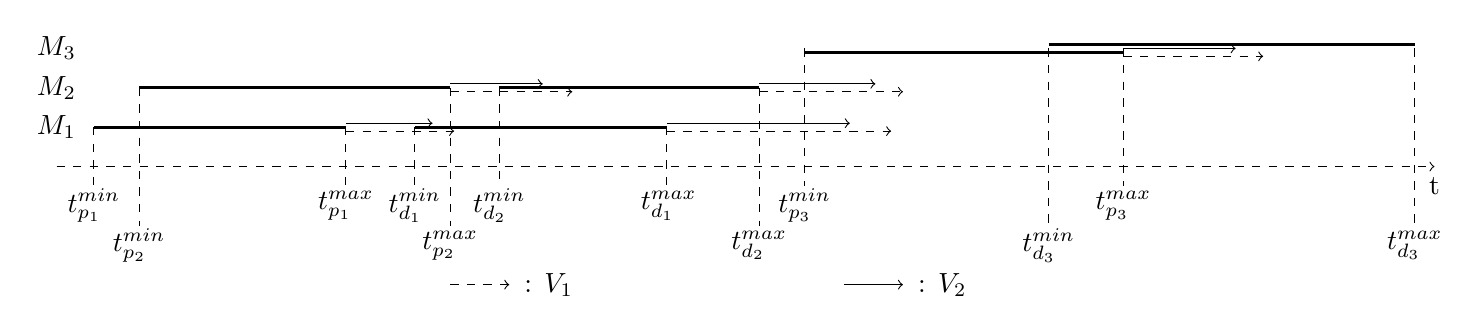
\begin{tikzpicture}[-,thick,xscale=0.25,yscale=0.5]
    \tikzstyle{v1}=[thin,dashed,->]
    \tikzstyle{v2}=[thin,->]
    \tikzstyle{tw}=[very thick,-,black]
    \tikzstyle{time}=[thin,dashed,->]
    \tikzstyle{trait}=[thin,dashed]

    \node (M1) at (5,1) {$M_1$};
    \node (M2) at (5,2) {$M_2$};
    \node (M3) at (5,3) {$M_3$};
    
    %M1
    \draw[tw] (6.9,1) -- (19.7,1);
    \draw[tw] (23.2,1) -- (36.0,1);
    %M2
    \draw[tw] (9.2,2) -- (25,2);
    \draw[tw] (27.5,2) -- (40.7,2);
    %M3
    \draw[tw] (43,2.9) -- (59.2,2.9);
    \draw[tw] (55.4,3.1) -- (74.0,3.1);

    %M1 : P -> D
    \draw[v1] (19.7,0.9) -- (25.2,0.9);
    \draw[v2] (19.7,1.1) -- (24.1,1.1);
    %M1 -> M3
    \draw[v1] (36,0.9) -- (47.4,0.9);
    \draw[v2] (36,1.1) -- (45.3,1.1);
    %M2 : P -> D
    \draw[v1] (25,1.9) -- (31.2,1.9);
    \draw[v2] (25,2.1) -- (29.7,2.1);
    %M2 -> M3
    \draw[v1] (40.7,1.9) -- (48,1.9);
    \draw[v2] (40.7,2.1) -- (46.6,2.1);
    %M3 : P -> D
    \draw[v1] (59.2,2.8) -- (66.3,2.8);
    \draw[v2] (59.2,3.0) -- (64.9,3);
    
    \draw[time] (5,0) -- (75.0,0);

    \draw[trait] (6.9,1) -- (6.9,-0.5);
    \draw[trait] (19.7,1) -- (19.7,-0.5);
    \draw[trait] (23.2,1) -- (23.2,-0.5);
    \draw[trait] (36,1) -- (36,-0.5);
    
    \draw[trait] (9.2,2) -- (9.2,-1.5);
    \draw[trait] (25,2) -- (25,-1.5);
    \draw[trait] (27.5,2) -- (27.5,-0.5);
    \draw[trait] (40.7,2) -- (40.7,-1.5);

    \draw[trait] (43,3) -- (43,-0.5);
    \draw[trait] (59.2,3) -- (59.2,-0.5);
    \draw[trait] (55.4,3) -- (55.4,-1.5);
    \draw[trait] (74,3) -- (74,-1.5);

    \node (m1PMin) at (6.9,-1) {$t_{p_1}^{min}$};
    \node (m1PMax) at (19.7,-1) {$t_{p_1}^{max}$};
    \node (m1DMin) at (23.2,-1) {$t_{d_1}^{min}$};
    \node (m1DMax) at (36.1,-1) {$t_{d_1}^{max}$};
    
    \node (m2PMin) at (9.2,-2) {$t_{p_2}^{min}$};
    \node (m2PMax) at (25,-2) {$t_{p_2}^{max}$};
    \node (m2DMin) at (27.5,-1) {$t_{d_2}^{min}$};
    \node (m2DMax) at (40.7,-2) {$t_{d_2}^{max}$};

    \node (m3PMin) at (43,-1) {$t_{p_3}^{min}$};
    \node (m3PMax) at (59.2,-1) {$t_{p_3}^{max}$};
    \node (m3DMin) at (55.4,-2) {$t_{d_3}^{min}$};
    \node (m3DMax) at (74,-2) {$t_{d_3}^{max}$};

    \node (t) at (75,-0.5) {t};

    \draw[v1] (25,-3) -- (28, -3);
    \draw[v2] (45,-3) -- (48,-3);

    \node (v1Legend) at (30, -3) { : $ V_1$ };
    \node (v2Legend) at (50, -3) { : $ V_2$ };
  \end{tikzpicture}
\end{center}


%===================================================
\section{ACO Graph}
%===================================================
\usetikzlibrary{patterns}
\tikzstyle{vertex}=[circle,fill=black!20,minimum size=25pt,inner sep=0pt,font=\tiny]
\tikzstyle{selected vertex} = [vertex, fill=black!20]
\tikzstyle{red vertex} = [vertex, fill=black!100, text=white]
\tikzstyle{blue vertex} = [vertex, fill=black!40]
\tikzstyle{edge} = [draw,thick,->]
\tikzstyle{weight} = [font=\small]
\tikzstyle{weightRed} = [font=\small, black!100]
\tikzstyle{weightBlue} = [font=\small, black!40]
\tikzstyle{red edge} = [draw,thick,->,red!100]
\tikzstyle{blue edge} = [draw,thick,->,blue!100]

\tikzstyle{ignored edge} = [draw,line width=5pt,-,black!20]

\vspace{10pt}

\begin{center}
\begin{tabular}{rl}

\multicolumn{2}{c}{
\begin{tikzpicture}[xscale=3, yscale=0.8, auto,swap]
    \foreach \pos/\name in {
	{(0,1)/source},
	{(1,2)/M1}, {(1,0)/M2},
	{(2,1)/M3},
	{(3,1)/sink}}
      \node[vertex] (\name) at \pos {$\name$};

    \foreach \source/ \dest /\weight in {source/M1/173, source/M2/334, M1/M3/636, M2/M3/407, M3/sink/348} \path[edge] (\source) -- node[weight] {$\weight$} (\dest);
    
    \foreach \vertex in {source,sink}
        \path node[selected vertex] at (\vertex) {$\vertex$};
\end{tikzpicture} }\\
\vspace{10pt}
t=$00:00:00$ & Distance graph.\\
\multicolumn{2}{c}{
\begin{tikzpicture}[xscale=3, yscale=0.8, auto,swap]
    \foreach \pos/\name in {
	{(0,1)/source},
	{(1,2)/M1}, {(1,0)/M2},
	{(2,1)/M3},
	{(3,1)/sink}}
      \node[vertex] (\name) at \pos {$\name$};

    \foreach \source/ \dest /\weightRed/\weightBlue in {source/M1/31/25, source/M2/60/48, M1/M3/114/92, M2/M3/73/59, M3/sink/63/50} \path[edge] (\source) -- node[weightRed,above] {$\weightRed$} node[weightBlue,below]{$\weightBlue$} (\dest);
    
    \foreach \vertex in {source,sink}
        \path node[selected vertex] at (\vertex) {$\vertex$};
    \foreach \vertex in {M2}
        \path node[red vertex] at (\vertex) {$\vertex$};
    \foreach \vertex in {M1,M3}
        \path node[blue vertex] at (\vertex) {$\vertex$};
\end{tikzpicture}} \\
\vspace{10pt}
t=$00:00:00$ & Colorized weighted graph after proccesing ACO. \\
\multicolumn{2}{c}{
\begin{tikzpicture}[xscale=3, yscale=0.8, auto,swap]
    \foreach \pos/\name in {
	{(0,1)/source},
	{(1,2)/M1},
	{(2,1)/M3},
	{(3,1)/sink}}
      \node[vertex] (\name) at \pos {$\name$};

    \foreach \source/ \dest /\weightRed/\weightBlue in {source/M1/324/25, M1/M3/73/59, M3/sink/63/50} \path[edge] (\source) -- node[weightRed,above] {$\weightRed$} node[weightBlue,below]{$\weightBlue$} (\dest);
    
    \foreach \vertex in {source,sink}
        \path node[selected vertex] at (\vertex) {$\vertex$};
    \foreach \vertex in {M1,M3}
        \path node[blue vertex] at (\vertex) {$\vertex$};
\end{tikzpicture}}\\
\vspace{10pt}
t=$00:00:32$ & $M_2$ startedd by $v_1$.\\ 
\multicolumn{2}{c}{
\begin{tikzpicture}[xscale=3, yscale=0.8, auto,swap]
    \foreach \pos/\name in {
	{(0,1)/source},
	{(2,1)/M3},
	{(3,1)/sink}}
      \node[vertex] (\name) at \pos {$\name$};

    \foreach \source/ \dest /\weightRed/\weightBlue in {source/M3/73/92, M3/sink/63/50} \path[edge] (\source) -- node[weightRed,above] {$\weightRed$} node[weightBlue,below]{$\weightBlue$} (\dest);
    
    \foreach \vertex in {source,sink}
        \path node[selected vertex] at (\vertex) {$\vertex$};
    \foreach \vertex in {M3}
        \path node[blue vertex] at (\vertex) {$\vertex$};
\end{tikzpicture}}\\
\vspace{10pt}
t=$00:00:34$ & $M_1$ startedd by $v_2$.\\
\multicolumn{2}{c}{
\begin{tikzpicture}[xscale=3, yscale=0.8, auto,swap]
    \foreach \pos/\name in {
	{(0,1)/source},
	{(3,1)/sink}}
      \node[vertex] (\name) at \pos {$\name$};

    \foreach \source/ \dest in {source/sink} \path[edge] (\source) -- (\dest);
    
    \foreach \vertex in {source,sink}
        \path node[selected vertex] at (\vertex) {$\vertex$};    
\end{tikzpicture}}\\
\vspace{10pt}
t=$00:06:47$ & $M_3$ startedd by $v_2$. \\
\multicolumn{2}{c}{
\begin{tikzpicture}[xscale=3, yscale=0.8, auto,swap]
\node[minimum size=5pt] (legend) at (1.25,-1) {$legend:$};    
\node[red vertex, minimum size=5pt] (v1legend) at (1.5,-1) {$V_1$};    
\node[blue vertex, minimum size=5pt] (v2legend) at (1.75,-1) {$V_2$};
\end{tikzpicture}}\\
\end{tabular}
\end{center}


% %===================================================
% \section{Time-distance incompatibilities}
% %===================================================
% 
% 
% Une des questions qui se posent est celle de la bonne modélisation du problème ou des différentes modélisations possibles. Je reparts d'un ensemble de missions $J$. Chaque mission $J_i$ est caractérisée par~:
% 
% \begin{itemize}
% \item un time window pour le pickup~: $W_{p_i} = [t_{p_i}^{min},t_{p_i}^{max}]$
% \item un time window pour le delivery~: $W_{d_i} = [t_{d_i}^{min},t_{d_i}^{max}]$
% \item un lieu de pickup $L_{p_i}$
% \item un lieu de delivery $L_{d_i}$ 
% \item un temps pour aller de $L_{p_i}$ à $L_{d_i}$~: $t_i$ 
% \end{itemize}
% 
% Je fais les hypothèses suivantes~: 
% 
% \begin{itemize}
% \item il n'y a aucun conflit pour l'accès à un lieu par un véhicule
% \item $t_i$ ne dépend pas du cavalier qui effectue la mission mais seulement des lieux $L_{p_i}$ et $L_{d_i}$
% \item $t_i$ reste identique quelle que soit la date à laquelle la mission est commencée
% \end{itemize}
% 
% 
% 
% %===================================================
% \section{Modèle Time-Interval}
% %===================================================
% 
% Considérons les deux time windows d'un job (en rouge) et le temps de déplacement (en bleu). Le temps de déplacement peut commencer à différentes dates tout en respectant les contraintes, c'est pour cela que j'ai indiqué plusieurs intervalles pour représenter le parcours. Mais on voit sur cet exemple qu'en cas d'un déplacement au plus tard (en vert), il reste plusieurs unités de temps pour le delivery ``en trop'' (je parle pour la version statique lorsqu'il n'y a aucune incertitude quant aux temps de déplacement), à moins que tu ne génères des time windows de longueur égale mais il n'y a a priori pas de raison. Je ne sais pas quoi faire de ce que je viens d'écrire. 
% 
% 
% \begin{center}
%   \begin{tikzpicture}[-,thick,xscale=0.4,yscale=0.4]
%     \tikzstyle{lastmove}=[very thick,-,green]
%     \tikzstyle{move}=[thick,-,blue]
%     \tikzstyle{tw}=[very thick,-,red]
%     \tikzstyle{time}=[thin,dashed,->]
%     
%     \draw[tw] (5,2) -- (8,2);
%     \draw[tw] (15,2) -- (20,2);
%     \draw[move] (5,3) -- (13,3);
%     \draw[move] (6,4) -- (14,4);
%     \draw[move] (7,5) -- (15,5);
%     \draw[lastmove] (8,6) -- (16,6);
% 
%     \draw[time] (0,0) -- (30,0);
%     
%   
%   \end{tikzpicture}
% \end{center}
% 
% 
% Je continue, considérons plusieurs jobs, ou plutôt plusieurs time windows associées à des jobs~:
% 
% 
% \begin{center}
%   \begin{tikzpicture}[-,thick,xscale=0.3,yscale=0.3]
%     \tikzstyle{lastmove}=[very thick,-,green]
%     \tikzstyle{move}=[thick,dashed,red]
%     \tikzstyle{tw}=[very thick,-,red]
%     \tikzstyle{time}=[thin,dashed,->]
%     
%     \draw[tw] (5,2) -- (7,2);
%     \draw[move] (7,2) -- (10,2);
%     \draw[tw] (10,2) -- (13,2);
% 
%     \draw[tw] (18,2) -- (21,2);
%     \draw[move] (21,2) -- (25,2);
%     \draw[tw] (25,2) -- (30,2);
% 
%     \draw[tw] (38,2) -- (41,2);
%     \draw[move] (41,2) -- (47,2);
%     \draw[tw] (47,2) -- (50,2);
% 
%     \draw[tw] (5,3) -- (8,3);
%     \draw[move] (8,3) -- (12,3);
%     \draw[tw] (12,3) -- (14,3);
% 
%     \draw[tw] (16,3) -- (18,3);
%     \draw[move] (18,3) -- (24,3);
%     \draw[tw] (24,3) -- (28,3);
% 
%     \draw[tw] (33,3) -- (36,3);
%     \draw[move] (36,3) -- (44,3);
%     \draw[tw] (44,3) -- (48,3);
% 
%     \draw[tw] (8,4) -- (12,4);
%     \draw[move] (12,4) -- (16,4);
%     \draw[tw] (16,4) -- (20,4);
% 
%     \draw[tw] (28,4) -- (32,4);
%     \draw[move] (32,4) -- (38,4);
%     \draw[tw] (38,4) -- (40,4);
% 
%     \draw[tw] (10,5) -- (12,5);
%     \draw[move] (12,5) -- (15,5);
%     \draw[tw] (15,5) -- (18,5);
% 
%     \draw[tw] (24,5) -- (27,5);
%     \draw[move] (27,5) -- (32,5);
%     \draw[tw] (32,5) -- (36,5);
% 
%     \draw[tw] (40,5) -- (42,5);
%     \draw[move] (42,5) -- (47,5);
%     \draw[tw] (47,5) -- (49,5);
% 
%     \draw[time] (0,0) -- (60,0);
%       
%   \end{tikzpicture}
% \end{center}
% 
% On peut aussi représenter les jobs de manière minimaliste en restreignant à l'inter-intervalle, ce qui donnerait ce qui est en dessous de la ligne pointillée~:
% 
% 
% \begin{center}
%   \begin{tikzpicture}[-,thick,xscale=0.3,yscale=0.3]
%     \tikzstyle{lastmove}=[very thick,-,green]
%     \tikzstyle{move}=[thick,dashed,red]
%     \tikzstyle{min}=[very thick,green]
%     \tikzstyle{tw}=[very thick,-,red]
%     \tikzstyle{time}=[thin,dashed,->]
%     \tikzstyle{ressources}=[thick,-]
%     \tikzstyle{trait}=[thin,dashed]
%     
%     \draw[tw] (5,2) -- (7,2);
%     \draw[move] (7,2) -- (10,2);
%     \draw[tw] (10,2) -- (13,2);
% 
%     \draw[tw] (18,2) -- (21,2);
%     \draw[move] (21,2) -- (25,2);
%     \draw[tw] (25,2) -- (30,2);
% 
%     \draw[tw] (38,2) -- (41,2);
%     \draw[move] (41,2) -- (47,2);
%     \draw[tw] (47,2) -- (50,2);
% 
%     \draw[tw] (5,3) -- (8,3);
%     \draw[move] (8,3) -- (12,3);
%     \draw[tw] (12,3) -- (14,3);
% 
%     \draw[tw] (16,3) -- (18,3);
%     \draw[move] (18,3) -- (24,3);
%     \draw[tw] (24,3) -- (28,3);
% 
%     \draw[tw] (33,3) -- (36,3);
%     \draw[move] (36,3) -- (44,3);
%     \draw[tw] (44,3) -- (48,3);
% 
%     \draw[tw] (8,4) -- (12,4);
%     \draw[move] (12,4) -- (16,4);
%     \draw[tw] (16,4) -- (20,4);
% 
%     \draw[tw] (28,4) -- (32,4);
%     \draw[move] (32,4) -- (38,4);
%     \draw[tw] (38,4) -- (40,4);
% 
%     \draw[tw] (10,5) -- (12,5);
%     \draw[move] (12,5) -- (15,5);
%     \draw[tw] (15,5) -- (18,5);
% 
%     \draw[tw] (24,5) -- (27,5);
%     \draw[move] (27,5) -- (32,5);
%     \draw[tw] (32,5) -- (36,5);
% 
%     \draw[tw] (40,5) -- (42,5);
%     \draw[move] (42,5) -- (47,5);
%     \draw[tw] (47,5) -- (49,5);
% 
%     \draw[time] (0,0) -- (60,0);
% 
%     \draw[min] (7,-2) -- (10,-2);
%     \draw[min] (21,-2) -- (25,-2);
%     \draw[min] (41,-2) -- (47,-2);
%     \draw[min] (8,-3) -- (12,-3);
%     \draw[min] (18,-3) -- (24,-3);
%     \draw[min] (36,-3) -- (44,-3);
%     \draw[min] (12,-4) -- (16,-4);
%     \draw[min] (32,-4) -- (38,-4);
%     \draw[min] (12,-5) -- (15,-5);
%     \draw[min] (27,-5) -- (32,-5);
%     \draw[min] (42,-5) -- (47,-5);
% 
%     \draw[min] (7,-2) -- (10,-2);
%     \draw[min] (21,-2) -- (25,-2);
%     \draw[min] (41,-2) -- (47,-2);
%     \draw[min] (8,-3) -- (12,-3);
%     \draw[min] (18,-3) -- (24,-3);
%     \draw[min] (36,-3) -- (44,-3);
%     \draw[min] (12,-4) -- (16,-4);
%     \draw[min] (32,-4) -- (38,-4);
%     \draw[min] (12,-5) -- (15,-5);
%     \draw[min] (27,-5) -- (32,-5);
%     \draw[min] (42,-5) -- (47,-5);
% 
%     \draw[trait] (7,-2) -- (7,-7);
%     \draw[trait] (21,-2) -- (21,-7);
%     \draw[trait] (41,-2) -- (41,-7);
%     \draw[trait] (8,-3) -- (8,-7);
%     \draw[trait] (18,-3) -- (18,-7);
%     \draw[trait] (36,-3) -- (36,-7);
%     \draw[trait] (12,-4) -- (12,-7);
%     \draw[trait] (32,-4) -- (32,-7);
%     \draw[trait] (27,-5) -- (27,-7);
%     \draw[trait] (42,-5) -- (42,-7);
%     \draw[trait] (10,-7) -- (10,-2);
%     \draw[trait] (25,-7) -- (25,-2);
%     \draw[trait] (47,-7) -- (47,-2);
%     \draw[trait] (12,-7) -- (12,-3);
%     \draw[trait] (24,-7) -- (24,-3);
%     \draw[trait] (44,-7) -- (44,-3);
%     \draw[trait] (16,-7) -- (16,-4);
%     \draw[trait] (38,-7) -- (38,-4);
%     \draw[trait] (15,-7) -- (15,-5);
%     \draw[trait] (32,-7) -- (32,-5);
% 
%     \node (a) at (3,-8) {0};
%     \node (b) at (7.5,-8) {1};
%     \node (c) at (9,-8) {2};
%     \node (d) at (11,-8) {1};
%     \node (e) at (13,-8) {2};
%     \node (f) at (15.5,-8) {1};
%     \node (g) at (17,-8) {0};
%     \node (h) at (19,-8) {1};
%     \node (i) at (22,-8) {2};
%     \node (j) at (24.5,-8) {1};
%     \node (k) at (26,-8) {0};
%     \node (l) at (30,-8) {1};
%     \node (m) at (34,-8) {1};
%     \node (n) at (37,-8) {2};
%     \node (p) at (39,-8) {1};
%     \node (q) at (41.5,-8) {2};
%     \node (r) at (43,-8) {3};
%     \node (s) at (46,-8) {2};
%     \node (t) at (50,-8) {0};
% 
%     \draw[ressources] (0,-7) -- (60,-7);
%       
%   \end{tikzpicture}
% \end{center}
% 
% Ce nombre donne le nombre minimum de ressources nécessaires, mais pas forcément suffisants pour respecter les contraintes. On peut ensuite ajouter les délais entre les tâches ce qui permet en plus d'ajouter des contraintes de précédence possibles entre les tâches. 

\end{document}

